\documentclass[draft=on]{scrbook}
\usepackage{blindtext}
\usepackage{clrscode3e}		%clrs package
\usepackage{graphicx}		%插入图片   

\begin{document}
\noindent
\begin{minipage}{.5\textwidth}
    \begin{codebox}
        \Procname{$\proc{rb-delete}(T,z)$} 
        \li    $y \gets z$
        \li    $\id{y-original-color} \gets \attrib{y}{color}$
        
        \li    \If $ \attrib{z}{left} \isequal \attrib{T}{nil} $
        \li        \Then  $ x  \gets \attrib{z}{right}$
        \li               $ \proc{rb-transplant}(T,z,\attrib{z}{right}) $
        \li    \ElseIf    $\attrib{z}{right} \isequal \attrib{T}{nil} $
        \li        \Then  $ x  \gets \attrib{z}{left} $
        \li               $ \proc{rb-transplant}(T,z,\attrib{z}{left}) $
        \li    \Else  $ y \gets \proc{tree-minimum}(\attrib{z}{right}) $
        \li           $ \id{y-original-color} \gets \attrib{y}{color} $  			  
        \li           $ x \gets \attrib{y}{right} $       
        \li           \If $ \attrib{y}{p} \isequal  z $		
        \li             \Then $ \attrib{x}{p}\gets y $
        \li           \Else  $ \proc{rb-transplant}(T,y,\attrib{y}{right}) $ 
        \li                  $ \attrib{y}{right} \gets \attrib{z}{right} $
        \li                  $ \attribb{y}{right}{p} \gets y $ 
        \End
        \li           $ \proc{rb-transplant}(T,z,y) $ 
        \li           $ \attrib{y}{left} \gets \attrib{z}{left} $ 
        \li           $ \attribb{y}{left}{p} \gets y $ 
        \li           $ \attrib{y}{color} \gets \attrib{z}{color} $ 
        \End
        
        \li    \If $ \id{y-original-color} \isequal \const{black} $
        \li       \Then $\proc{rb-delete-fixup}(\attrib{T}{x})$
        \End
      \end{codebox}
\end{minipage}% This must go next to `\end{minipage}`
\begin{minipage}{.5\textwidth}
    \begin{figure}[h] %figure环境,h默认参数是可以浮动,不是固定在当前位置。如果要不浮动,你就可以使用大写float宏包的H参数,固定图片在当前位置,禁止浮动。
		%\centering %使图片居中显示
		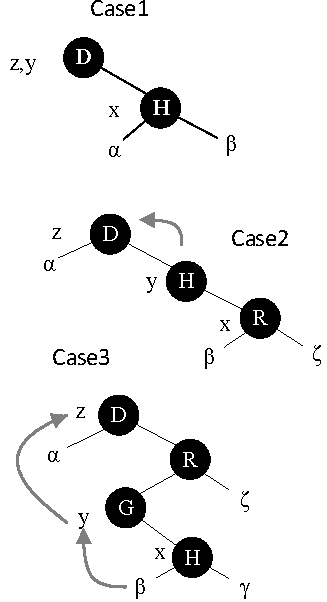
\includegraphics[width=0.4\textwidth]{vector/red-black-tree/delete/rb_delete_cases_single.pdf} %中括号中的参数是设置图片充满文档的大小,你也可以使用小数来缩小图片的尺寸。
		\caption{\noindent{The} simple delete cases .  } %caption是用来给图片加上图题的
		\label{rb_delete_cases_single} %这是添加标签,方便在文章中引用图片。
	\end{figure}%figure环境
\end{minipage}

AAAAAAAAAAAAAAAAAAAAASSSSSSSS SSSSSSS SSSSSSSSSSSS SSSSS
\end{document}